\documentclass{report}
\usepackage[utf8]{inputenc}
\usepackage{amsmath, amssymb}
\usepackage{graphicx}
\usepackage[margin=1.25in]{geometry}
\usepackage{multirow}
\usepackage{pdfpages}
\usepackage{float}
\usepackage{hyperref}
\hypersetup{
    colorlinks,
    citecolor=black,
    filecolor=black,
    linkcolor=black,
    urlcolor=black
}
\title{Lab \#6: Diffraction \& Interference Python Plotting}
\author{Neil Sawhney}
\date{December 2021}

\makeatletter
\def\@makechapterhead#1{%
  \vspace*{50\p@}% <----------------- Space from top of page to Chapter #
  {\parindent \z@ \raggedright \normalfont
    \ifnum \c@secnumdepth >\m@ne
        \huge\bfseries \thechapter.\ % <-- Chapter # (without "Chapter")
    \fi
    \interlinepenalty\@M
    #1\par\nobreak% <------------------ Chapter title
    \vskip 40\p@% <------------------ Space between chapter title and first paragraph
  }}
\makeatother
\begin{document}

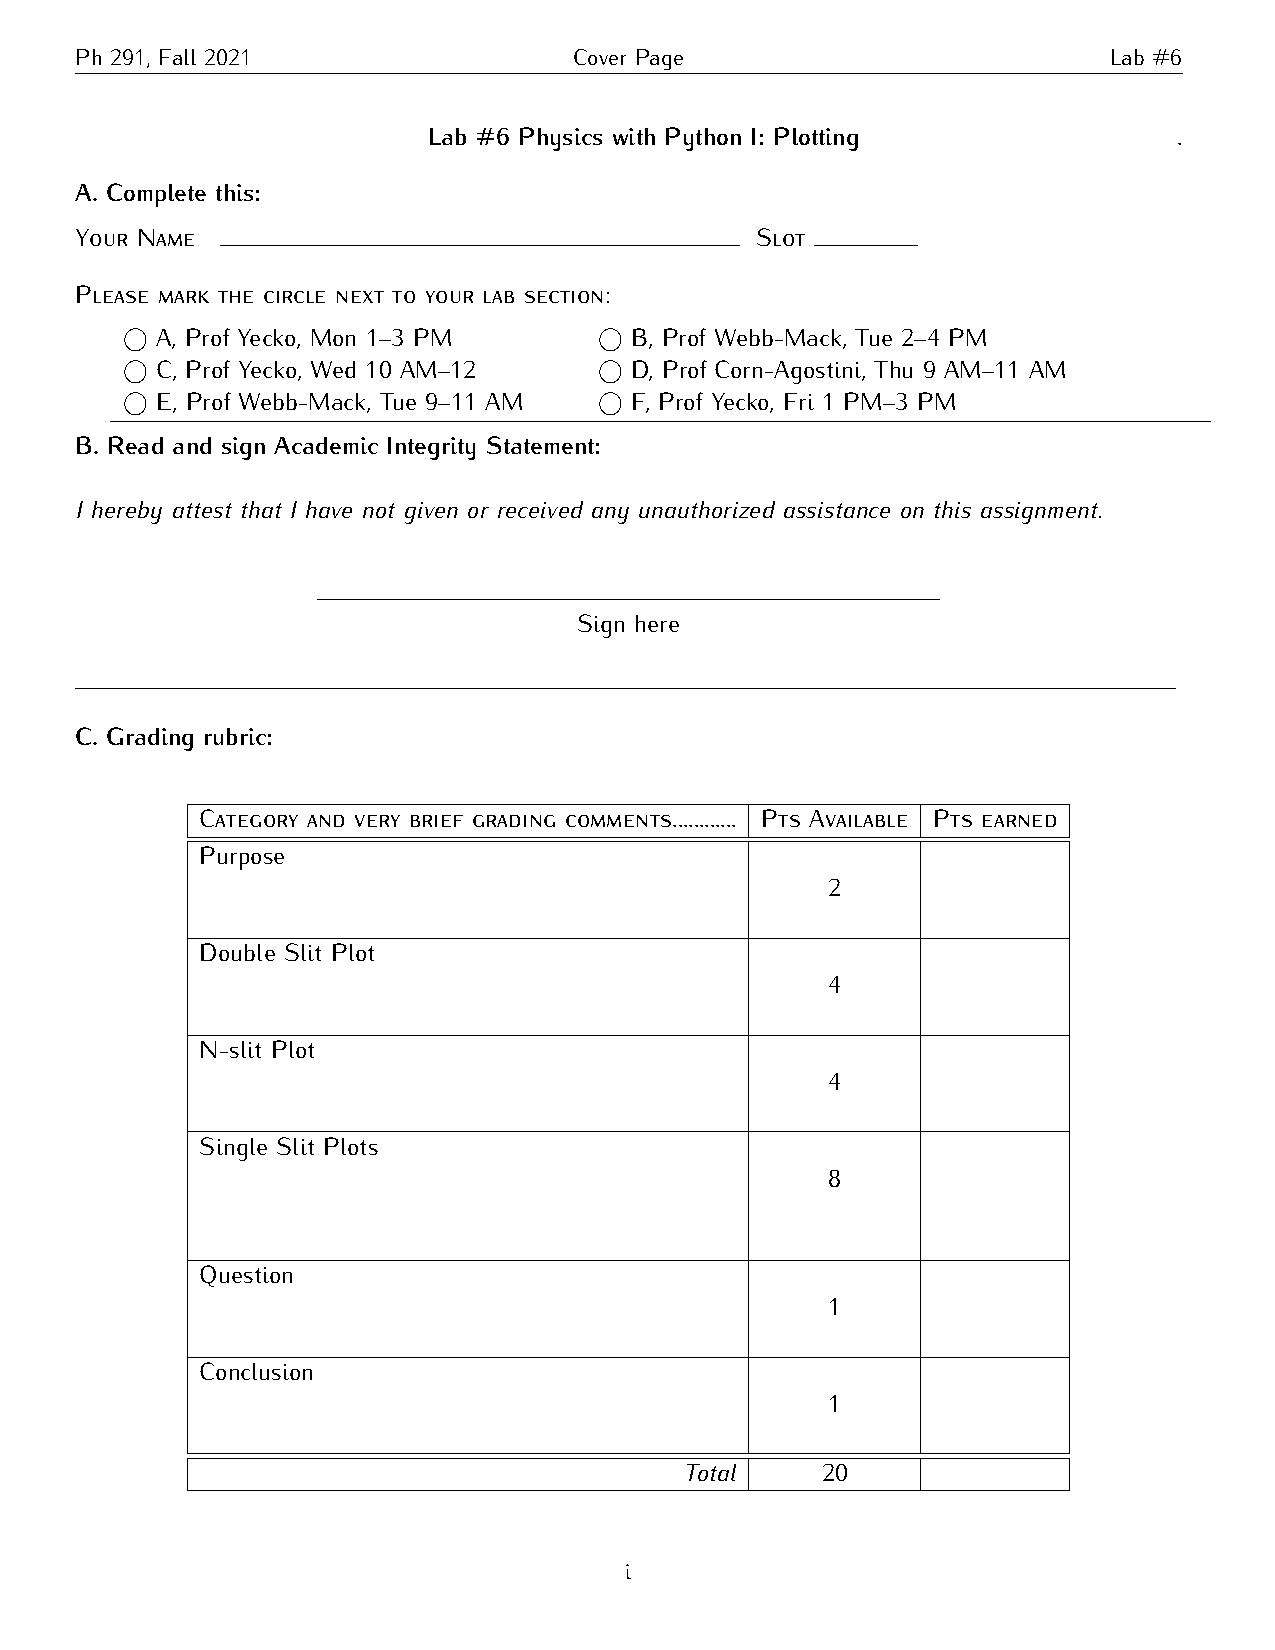
\includepdf[pages=-]{Lab6-COVER.pdf}

\maketitle
\tableofcontents

\chapter{Purpose}
The purpose of this lab is to plot the interference pattern of light as it passes through 1, 2, and N number of slits for both an infinitesimally small slit and a fixed width slit. 


%-----------------------------------

\chapter{Results}

\begin{table}[H]
    \centering
    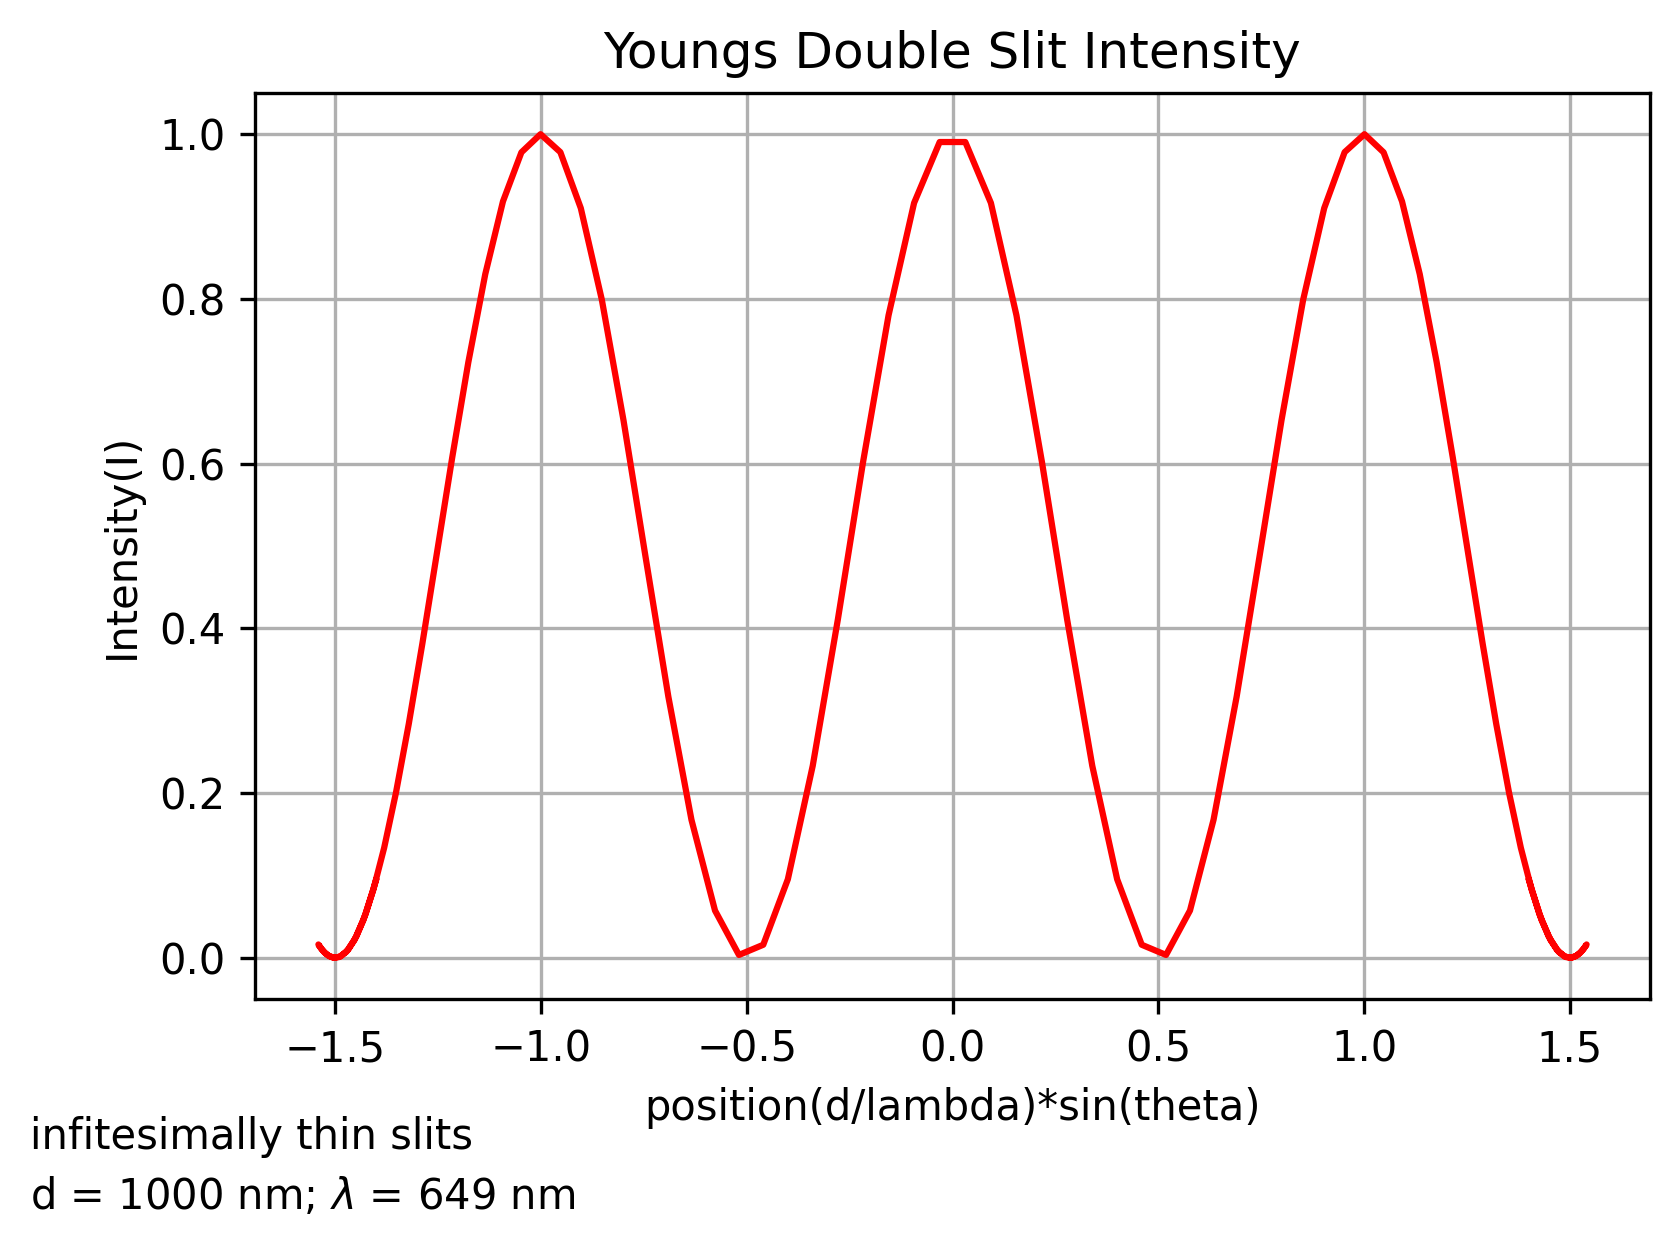
\includegraphics[width = \textwidth]{plot1.png}
    \caption{Diffraction Grating}
\end{table}
\bigskip

\begin{table}[H]
    \centering
    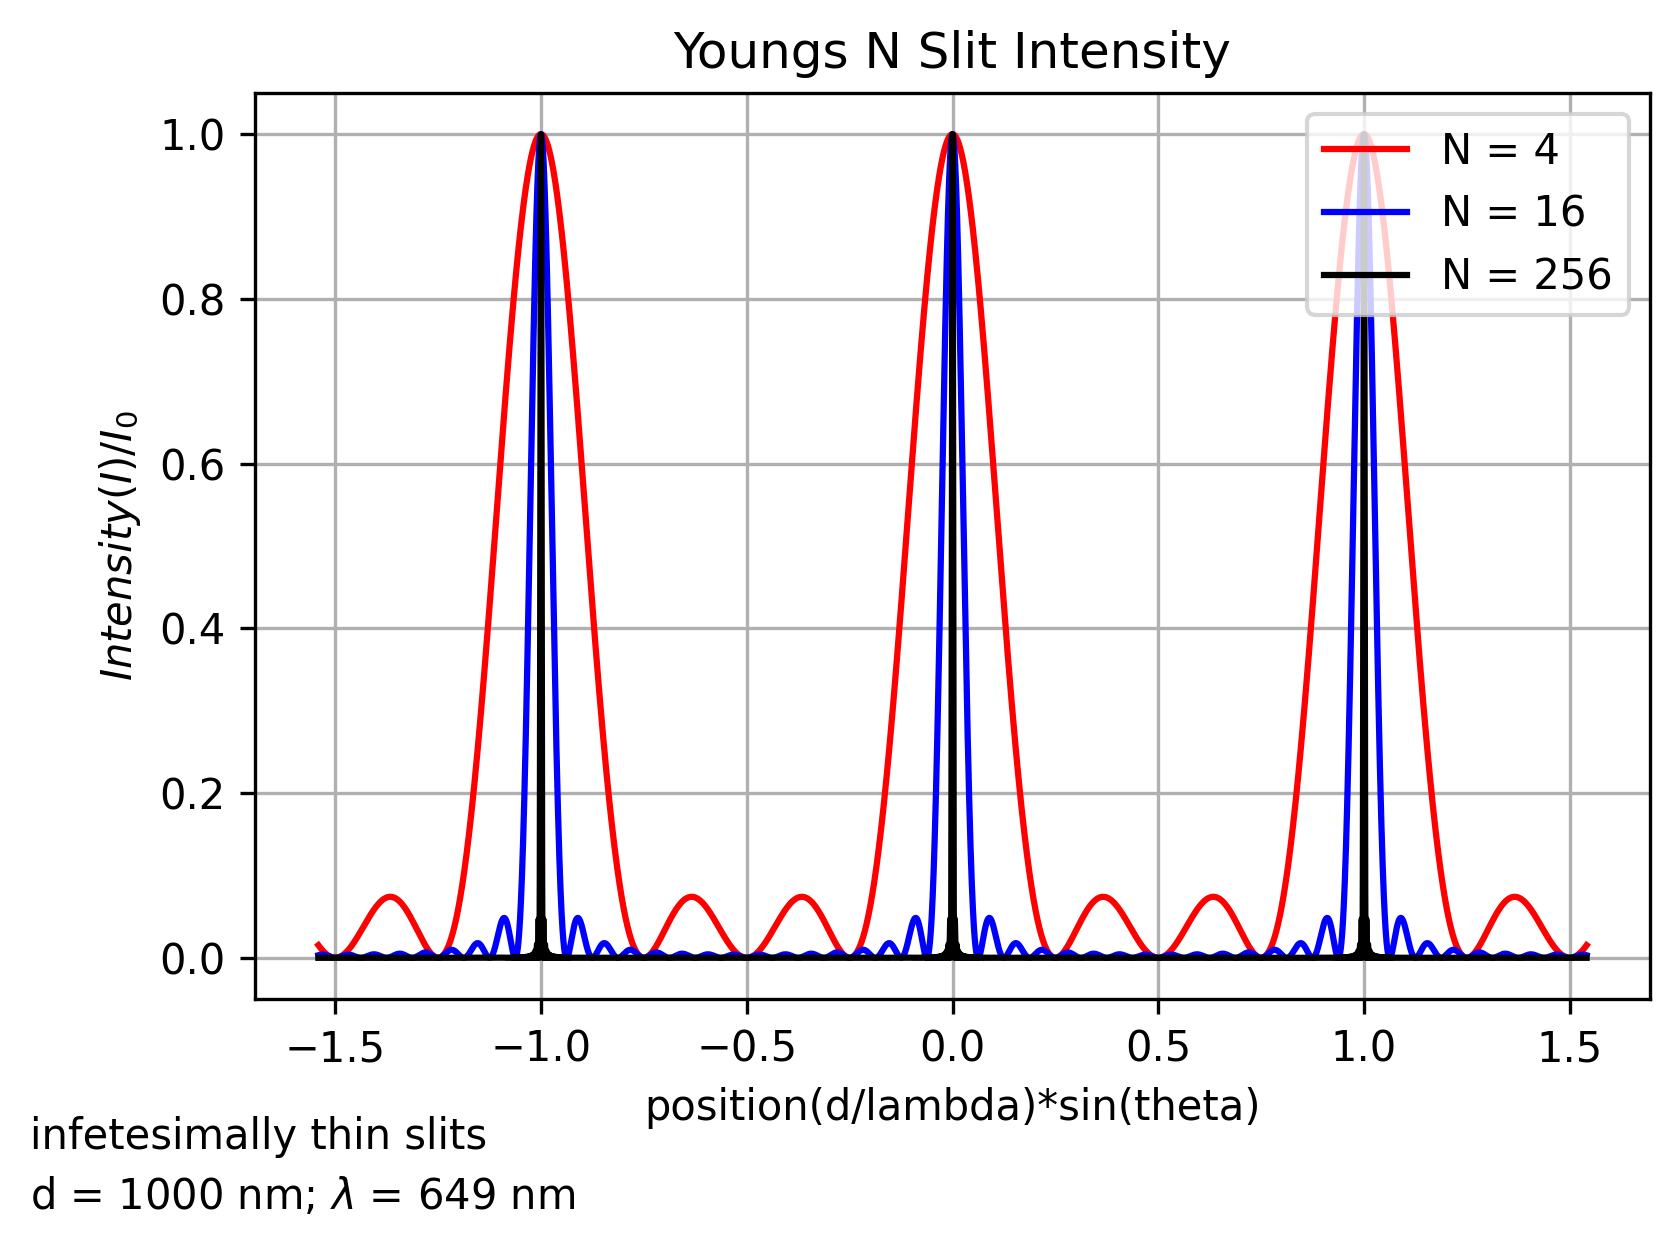
\includegraphics[width = \textwidth]{plot2.png}
    \caption{Diffraction Grating}
\end{table}
\bigskip

\begin{table}[H]
    \centering
    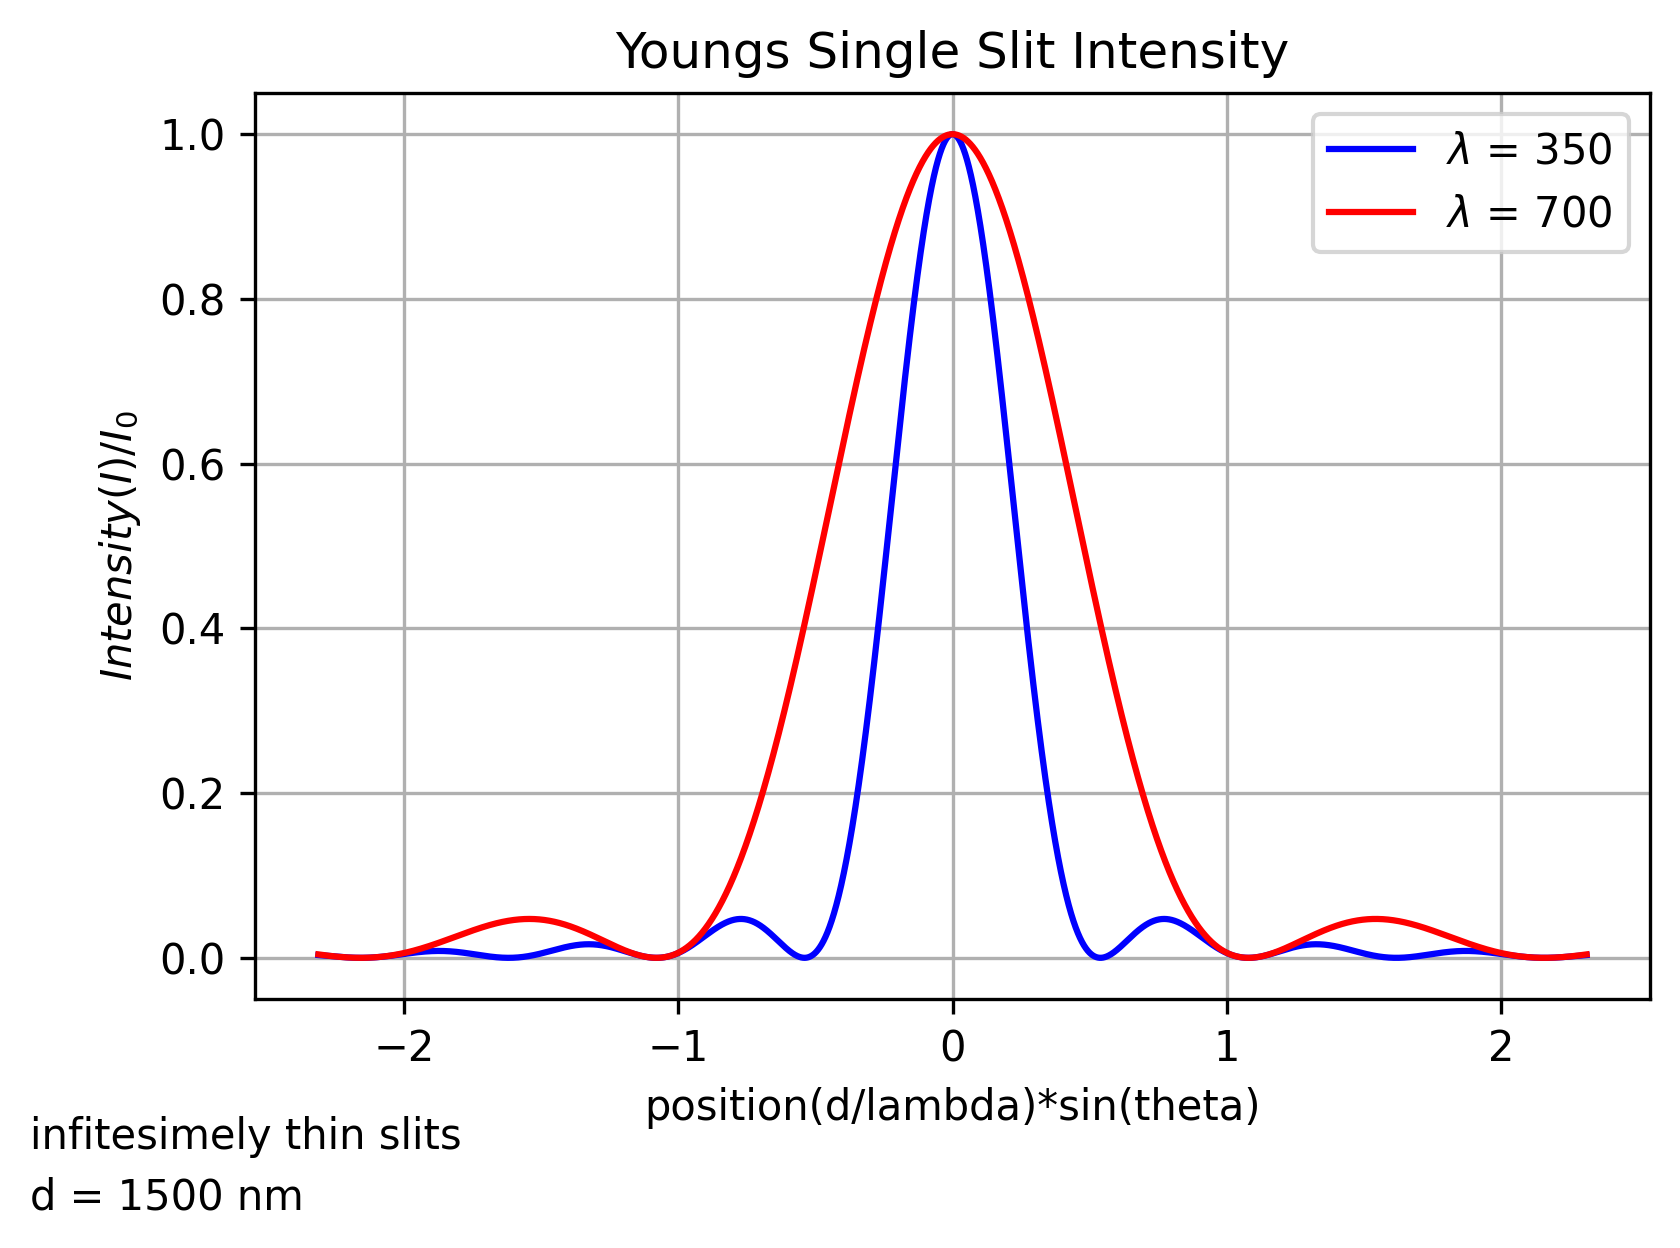
\includegraphics[width = \textwidth]{plot3.png}
    \caption{Diffraction Grating}
\end{table}
\bigskip

\begin{table}[H]
    \centering
    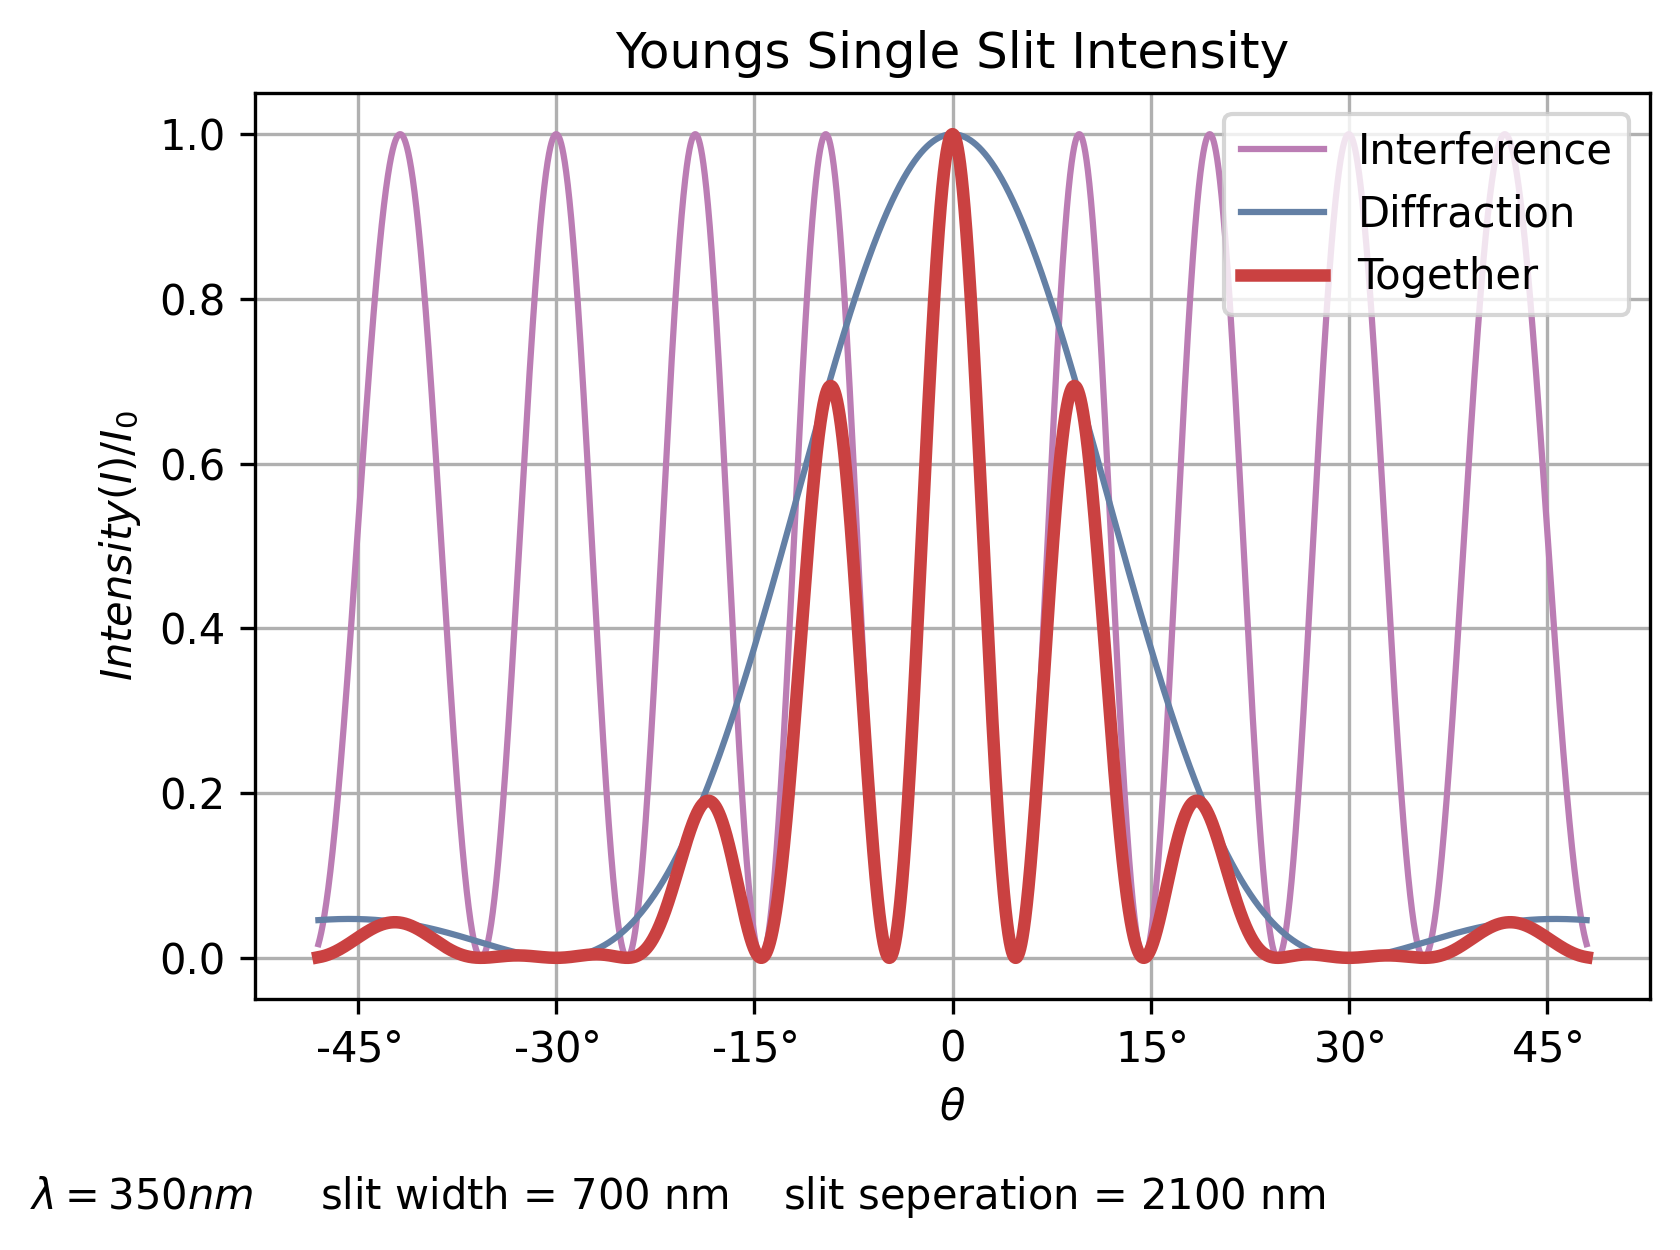
\includegraphics[width = \textwidth]{plot4.png}
    \caption{Diffraction Grating}
\end{table}
\bigskip

\subsection*{Question}

\chapter{Conclusions}

By using the interference and wave like nature of light, the diffraction pattern created by a laser hitting a hair was used to determine the thickness of the hair. The error bounds of the calculated value agrees with literature values.  




\chapter{Answered Questions}
Click the question to be brought to the location where the question is answered.

\section{Question}
\hyperref[Question]{missing m = 3 order}

\end{document}
